\section{Robust Scenario-Based Probabilistic Safety Verification Method}\label{sec:scenario-based_method}
\vspace{-0.5em}
Here, we propose a robust scenario-based probabilistic safety verification method for neural reachable tubes.
The new method is a straightforward application of a scenario-based sampling-and-discarding approach to chance-constrained optimization problems, which quantifies the trade-off between feasibility and performance of the optimal solution based on finite samples \citep{campi2011sampling}.
First, we explain the method when $\targetset$ represents undesirable states. In the end, we comment on when $\targetset$ represents desirable states. 

\noindent \textit{\textbf{Procedures:}}
Let $\safeset \subseteq X$ be a neural safe set that is, in the avoid case, the \textit{complement} of the neural reachable tube being verified.
In our case, $\safeset$ is typically a super-$\delta$ level set of the learned value function $\Tilde{\vfunc}(\state,0)$.
Ideally, any super-$\delta$ level set of $\Tilde{\vfunc}(\state,0)$ for $\delta > 0$ should be a valid safe set; however, due to learning errors, that might not be true in practice.
To provide a probabilistic safety assurance for $\safeset$, we first sample $N$ independent and identically distributed (i.i.d.) states $x_{1:N}$ from $\safeset$ according to some probability distribution $\mathbb{P}$ over $\safeset$.
Since $\safeset$ is defined implicitly by $\Tilde{\vfunc}(\state,0)$, we use rejection sampling.
We next compute the costs $\costFunction(\state_i,0)$ for $i=1, 2, ..., N$ by rolling out the system trajectory from $x_i$ under $\Tilde{\policy}(x,t)$.
Let $k$ refer to the number of ``outliers'' - samples that are empirically unsafe, i.e., $\costFunction(\state_i,0) \le 0$.
Then the following theorem provides a probabilistic guarantee on the safety of the neural reachable tube and its complement, the neural safe set $\safeset$: 
%Then the following theorem provides a probabilistic guarantee on the safety of the neural reachable tube and its complement, the neural safe set $\safeset$, which we prove in \appendixref{apd:scenario-based_theorem_proof}:
% 
\vspace{-0.5em}
\begin{theorem}[Robust Scenario-Based Probabilistic Safety Verification]
    \label{theorem:scenario-based_method}
    Select a safety violation parameter $\epsilon \in (0, 1)$ and a confidence parameter $\beta \in (0, 1)$ such that
    \vspace{-0.5em}
    \begin{equation} \label{eq:theorem_parameters_relationship}
        \begin{aligned}
            \sum^k_{i=0} \binom{N}{i} \epsilon^i (1-\epsilon)^{N-i} \le \beta
        \end{aligned}
    \end{equation}
    where $k$ and $N$ are as defined above. 
    Then, with probability at least $1-\beta$, the following holds:
    \begin{equation} \label{eq:robust_guarantee}
        \begin{aligned}
            \underset{\state \in \safeset}{\mathbb{P}} \left( \vfunc(\state,0) \le 0 \right) \le \epsilon
        \end{aligned}
    \end{equation}
\end{theorem}
% 
All proofs can be found in the Appendix of the extended version of this article\footnote{\label{note:extended_paper}See \url{https://sia-lab-git.github.io/Verification_of_Neural_Reachable_Tubes.pdf}}.
Disregarding the confidence parameter $\beta$ for a moment, \theoremref{theorem:scenario-based_method} states that the fraction of $\safeset$ that is unsafe is bounded above by the violation parameter $\epsilon$, where $\epsilon$ is computed empirically using Equation \eqref{eq:theorem_parameters_relationship} based on the outlier rate $k$ encountered within $N$ samples.
$\epsilon$ is thus a reflection of the safety quality of $\safeset$, which degrades with the increase in the number of outliers $k$, as expected. This can also be seen for the running example in \figureref{fig:fixed_N} (the red curve).
Overall, \theoremref{theorem:scenario-based_method} allows us to compute probabilistic safety guarantees for any neural set $\safeset$ based on a finite number of samples.
Subsequently, this result can be used to find some $\safeset$ for which $\epsilon$ is smaller than a desired threshold, as we discuss later in this section.

To interpret $\beta$, note that $k$ is a random variable that depends on the randomly sampled $x_{1:N}$. It may be the case that we just happen to draw an unrepresentative sample, in which case the $\epsilon$ bound does not hold. $\beta$ controls the probability of this adverse event happening, which regards the correctness of the probabilistic safety guarantee in Equation \eqref{eq:robust_guarantee}. Fortunately, $\beta$ goes to $0$ exponentially with $N$, so $\beta$ can be chosen to be an extremely small value, such as $10^{-16}$, when we sample large $N$. $1-\beta$ will then be so close to $1$ that it does not have any practical importance.

We have just explained the robust scenario-based probabilistic safety verification method in the case where $\targetset$ represents undesirable states. When the system instead wants to reach $\targetset$, $\safeset$ will be a sublevel set instead of a superlevel set of the learned value function.
The cost inequality should be flipped when computing $k$, and the value inequality should be flipped in Equation \eqref{eq:robust_guarantee}. 

\subsection{Comparison of Robust and Iterative Scenario-Based Probabilistic Safety Verification}\label{sec:comparison}
\vspace{-0.5em}
The key difference between the proposed robust scenario-based method and the iterative scenario-based method discussed in \sectionref{sec:deepreach_iterative_verification} is that the former can handle nonzero empirical safety violations $k$.
This enables several crucial advantages that we demonstrate in \figureref{fig:fixed_N,fig:diff_N} for a solution learned by DeepReach on the multi-vehicle collision avoidance running example in \sectionref{sec:problem_setup}. We have fixed the confidence parameter $\beta = 10^{-16}$ to be so close to $0$ that it has no practical significance ($\beta$ plays the same role in both methods).
% 
\vspace{-0.5em}
\begin{figure}[h!]
    \begin{minipage}[c]{0.32\textwidth}
       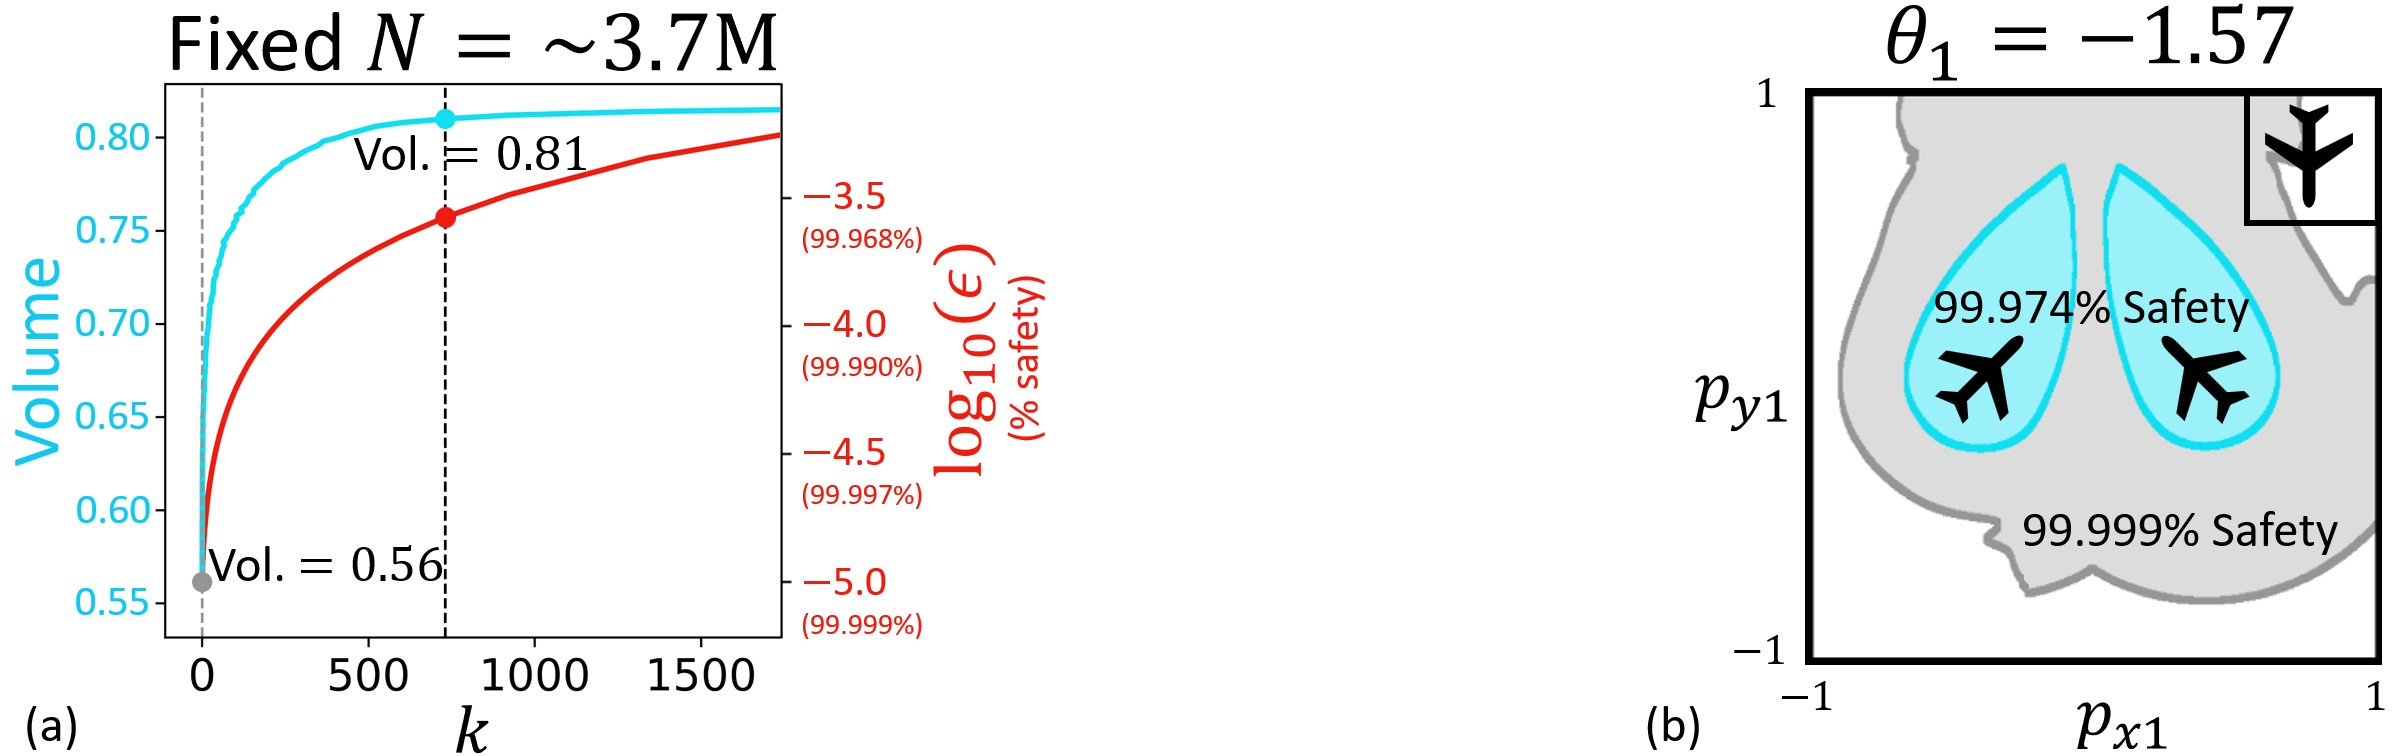
\includegraphics[trim={0 0 35cm 0},clip, width=\textwidth]{figures/Figure_1}

        \vspace{0.5em}
       
        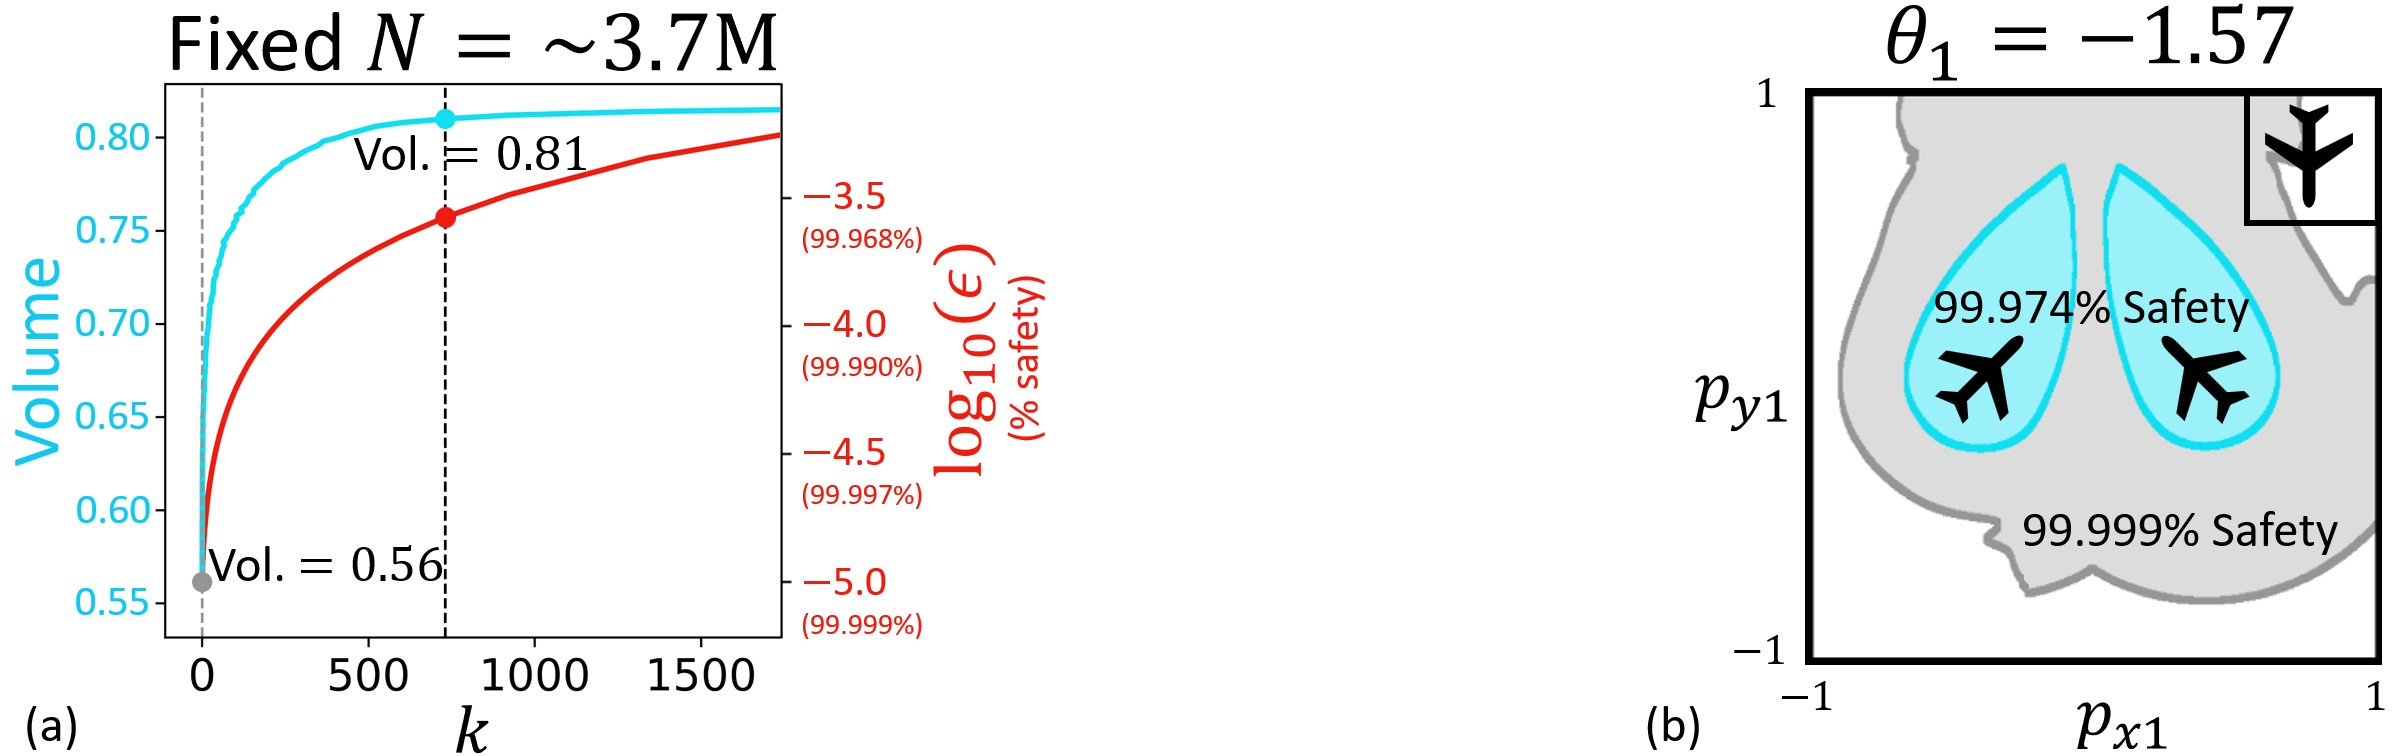
\includegraphics[trim={43cm 0 0 0},clip, width=0.75\textwidth]{figures/Figure_1}
    \end{minipage}\hfill
    \begin{minipage}[c]{0.67\textwidth}
        \caption{(Top) For a fixed simulation budget $N$, the cyan curve shows the number of empirical safety violations $k$ for different learned volumes (different super-levels of $\Tilde{\vfunc}(\state,0)$). The red curve shows the trade-off in safety strength $\epsilon$ (in log scale) for each $k$ using the robust method. The grey point indicates the iterative method baseline. The robust method is able to provide safety assurances even for the volumes that have non-zero outliers. (Dashed black line) By a small decrease in safety level (from $99.999\%$ to $99.974\%$) caused by outliers, we are able to significantly increase the assured safe volume from $0.56$ to $0.81$. (Bottom) Correspondingly, the safe set $\safeset$ increases greatly from the complement of the grey region to the complement of the blue region.} \label{fig:fixed_N}
    \end{minipage}
    \vspace{-1.0em}
\end{figure}
% 

Firstly, for a fixed simulation budget $N$, the robust method allows one to trade off the probabilistic strength of safety (increasing $\epsilon$) for resilience (increasing $k$).
In other words, the method can verify any given neural safe set $\safeset$ in an outlier-robust fashion by automatically attenuating the level of safety assurance based on the number of empirical outliers (i.e., safety violations).
The iterative method, in contrast, can only verify a region that is outlier-free.
Consequently, the robust method enables one to engage in a trade-off if a large increase in safe set volume can be attained by a tolerable decrease in safety, as illustrated in \figureref{fig:fixed_N}.
% % 
% \begin{figure}[htbp]
%     \centering
%     \includegraphics[width=1.0\columnwidth]{figures/Figure 1}
%     \caption{(Left) For a fixed simulation budget $N$, the cyan curve shows the number of empirical safety violations $k$ for different learned volumes (different super-levels of $\Tilde{\vfunc}(\state,0)$). The red curve shows the trade-off in safety strength $\epsilon$ (in log scale) for each $k$ using the robust method. The grey point indicates the iterative method baseline. The robust method is able to provide safety assurances even for the volumes that have non-zero outliers. (Dashed black line) By a small decrease in safety level (from $99.999\%$ to $99.974\%$) caused by outliers, we are able to significantly increase the assured safe volume from $0.56$ to $0.81$. (Right) The $\BRT$, the complement of the safe set $\safeset$, shrinks greatly (from grey to blue).}
%     %\vspace{-2.0em}
%     \label{fig:fixed_N}
% \end{figure}
% % 
% % 
% \begin{SCfigure}
%     \centering
%     \includegraphics[trim={0 0 35cm 0},clip, width=0.4\columnwidth]{figures/Figure 1}
%     \caption{(Left) For a fixed simulation budget $N$, the cyan curve shows the number of empirical safety violations $k$ for different learned volumes (different super-levels of $\Tilde{\vfunc}(\state,0)$). The red curve shows the trade-off in safety strength $\epsilon$ (in log scale) for each $k$ using the robust method. The grey point indicates the iterative method baseline. The robust method is able to provide safety assurances even for the volumes that have non-zero outliers. (Dashed black line) By a small decrease in safety level (from $99.999\%$ to $99.974\%$) caused by outliers, we are able to significantly increase the assured safe volume from $0.56$ to $0.81$. (Right) The $\BRT$, the complement of the safe set $\safeset$, shrinks greatly (from grey to blue).}
%     %\vspace{-2.0em}
%     \label{fig:fixed_N}
% \end{SCfigure}
% % 
% 
% 
% 
\vspace{-0.5em}
\begin{figure}[h!]
    \centering
    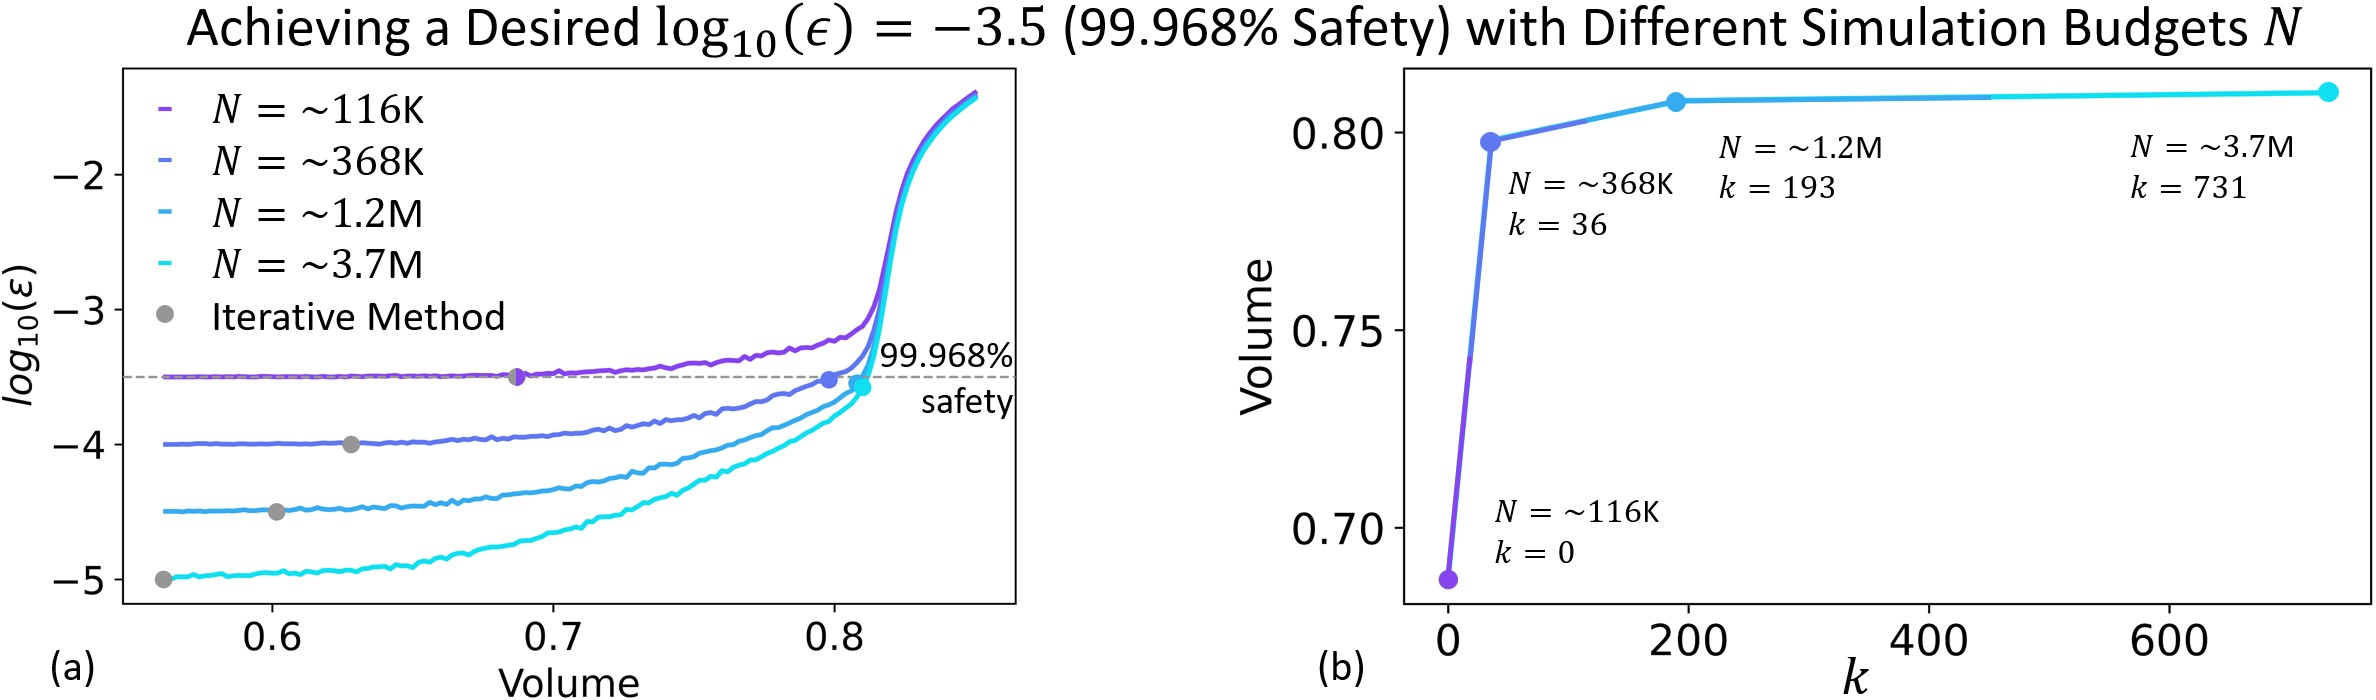
\includegraphics[width=0.95\columnwidth]{figures/Figure_2}
    \vspace{-0.5em}
    \caption{(Left) Computing the safety strength $\epsilon$ across different volumes (different super-levels of $\Tilde{\vfunc}(\state,0)$) for different simulation budgets $N$ using the robust method. The grey points indicate the iterative method baselines. (Right) As we increase $N$, the largest volume achieving the desired $99.968\%$ safety using the robust method increases up to a limit.}
    \vspace{-1em}
    \label{fig:diff_N}
\end{figure}
% 

Secondly, by allowing nonzero safety violations $k$, the robust method provides stronger safety assurances for a \textit{fixed} volume with increment in the simulation budget $N$, as long as the outlier rate does not grow substantially with $N$.
Thus, with more simulation effort, significantly larger volumes can be attained \textit{for a desired safety strength $\epsilon$} as shown in \figureref{fig:diff_N}.
Incrementing $N$ in the iterative method, on the other hand, will only correspond to verifying \textit{smaller} volumes at a \textit{stronger} $\epsilon$.
It cannot verify larger volumes for a fixed $\epsilon$, because empirical safety violations will be introduced.
\figureref{fig:diff_N} shows how the robust method (curves) adds a new degree of freedom for computing safety assurances compared to the iterative method (grey points).

